\chapter{Management process}
\section{Project start plan}
In deze sectie bespreken we de verwachte kost van het project. Voor de kostberekening maken we gebruik van het COCOMO I model. Als type project kiezen we tussen ``simple'', ``semidetached'' en ``embedded''. We kiezen hierin voor het type ``semidetached''. Dit weerspiegelt goed de huidige situatie van ons team. De omvang ons team is aan de grote kant en er zijn veel onbekende factoren in dit project (zie ook \ref{sec:risicoManagementPlan}). We gebruiken dan volgende formule:
\begin{equation*}
	E = a*KLOC^b
\end{equation*}
Hierbij is $E$ de ``effort'' uitgedrukt in persoonsmaanden (pm). Voor ons is het echter interessanter om naar de werkuren te kijken. Volgens de COCOMO standaard bevat \'{e}\'{e}n werkmaand 152 uren.  De benodigde tijd ($T$) kan dan als volgt berekend worden:
\begin{equation*}
	T = 152\frac{u}{pm}*E
\end{equation*}
Hierbij wordt T uitgedrukt in uren. Uit de tabellen van het COCOMO-model volgt dat $a = 3.0$ en $b = 1.12$. Verder schatten we in dat dit project een totale omvang zal hebben van 10KLOC. Dit geeft dan:
\begin{equation*}
	T = 152*3.0*10^{1.12} \approx 6011u 
\end{equation*}
Vermits ons team uit 7 personen bestaat, geeft dit per persoon een tijdsduur van:
\begin{equation*}
	T_{persoon} \approx 859u
\end{equation*}
Het spreekt voor zich dat dit duidelijk een overschatting is. $859u$ 
\section{Werk plan} \label{sec:workplan}
\subsection{Activiteiten}
Het project bestaat uit volgende activiteiten\footnote{In volgende versies van het SPMP komen hier nog verscheidene activiteiten bij.}, weergegeven als een work breakdown structure in figuur \ref{fig:workbreakdownstructure}.
\begin{figure} [H]
    \centering
    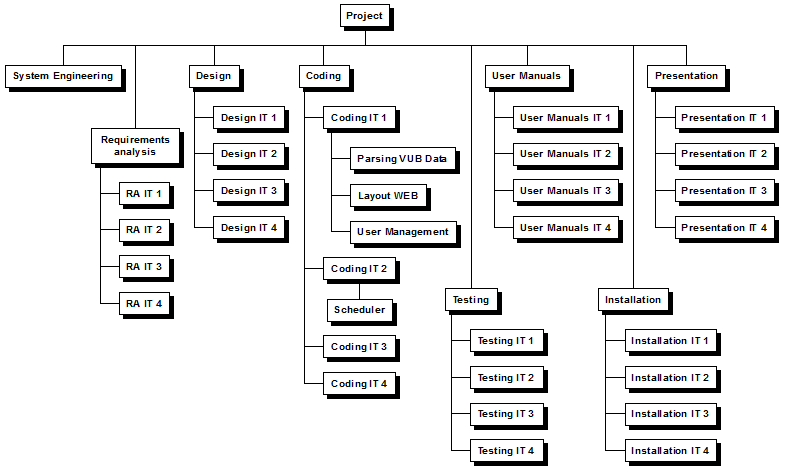
\includegraphics[width = \textwidth]{ManagerialProcess/WBSChart.png}
    \caption{Work breakdown structure.}
	\label{fig:workbreakdownstructure}
\end{figure}
Voor de eerste iteratie is de work breakdown structure weergegeven in figuur \ref{fig:wbsIteratie1}.
\begin{figure} [H]
	\centering
	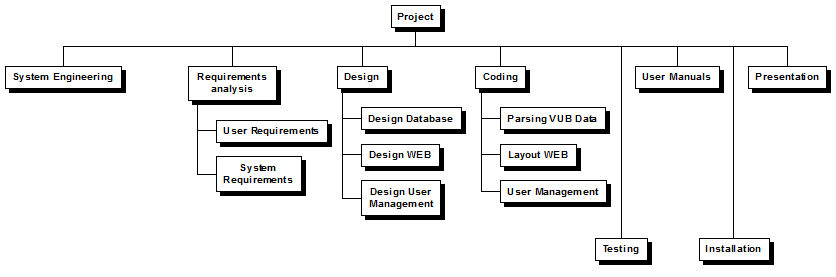
\includegraphics[width = \textwidth]{ManagerialProcess/WBSChartIteratie1.png}
	\caption{Work breakdown structure van iteratie 1.}
	\label{fig:wbsIteratie1}
\end{figure}
In de volgende versies van de SPMP zullen de work breakdown structures van de volgende iteraties worden weergegeven.
\subsection{Planning}
In tabel \ref{tab:ActivityDependenciesIteratie1} is een overzicht weergegeven van de verschillende activiteiten gedurende iteratie 1. Hierbij zijn ook de afhankelijkheden weergegeven tussen deze activiteiten. Op basis van deze tabel kunnen we een Gantt chart opstellen en het kritisch pad bepalen.
\begin{table} [H]
	\centering
	\caption{Activiteiten van de eerste iteratie en afhankelijkheden.}
	\begin{tabular} {c|l|c|c}
		Activiteit ID & Activiteit Naam & Tijdsduur (in dagen) & Afhankelijkheden \\
		\hline
		1 & System Engineering & 21 & \\
		2 & Requirements Analysis & 14 & \\
		2.1 & User Requirements & 7 & \\
		2.2 & System Requirements & 7 & 2.1 \\
		3 & Design & 14 & 2 \\
		3.1 & Design Database & 5 & \\
		3.2 & Design WEB & 4 & \\
		3.3 & Design User Management & 5 & \\
		4 & Coding & 14 & \\
		4.1 & Coding Parsing VUB Data & 7 & 3.1, Release data dump \\
		4.2 & Coding Layout WEB & 14 & 3.2 \\
		4.3 & Coding User Management & 14 & 3.3 \\
		5 & Testing & 7 & 4 \\
		6 & User manuals & 3 & 4 \\
		7 & Installation & 1 & 5,6 \\
		8 & Presentation & 3 & 7	
	\end{tabular}
	\label{tab:ActivityDependenciesIteratie1}
\end{table}
Op basis van tabel \ref{tab:ActivityDependenciesIteratie1} bekomen we de Gantt chart voor iteratie 1 weergegeven in figuur \ref{fig:GantChartIT1}. Het kritisch pad is weergegeven in het rood. Hierbij is nog rekening met extra constraints:
\begin{itemize}
	\item Het project is gestart op 7 oktober 2013.
	\item De activiteit ``Requirements Analysis'' kan niet vroeger beginnen dan 21 oktober 2013.
	\item De activiteit ``Parsing VUB Data'' kan niet vroeger beginnen dan 18 november 2013 (zie tabel \ref{tab:kalender}).
	\item De activiteit ``Installation'' mag niet later eindigen dan 13 december 2013 (zie tabel \ref{tab:kalender}).
	\item De activiteit ``Presentation'' mag niet later eindigen dan 18 december 2013 (zie tabel \ref{tab:kalender}).
\end{itemize}
\begin{figure} [H]
	\centering
	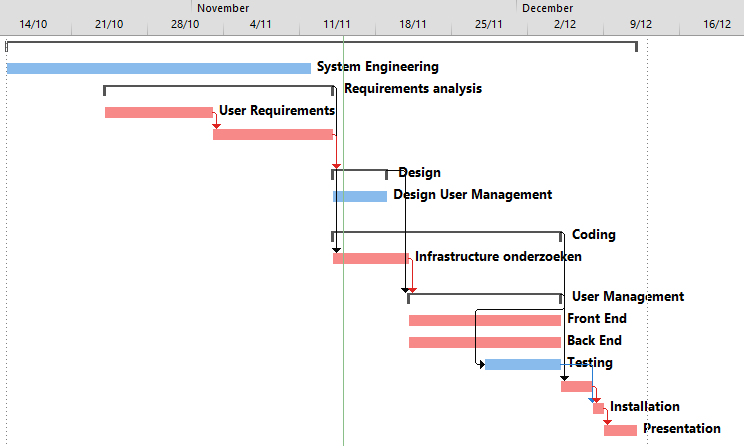
\includegraphics[width = \textwidth]{ManagerialProcess/GanttChartIT1.png}	
	\caption{Gantt chart voor iteratie 1.}
	\label{fig:GantChartIT1}
\end{figure}
Het kritisch pad begint bij de activiteit ```Parsing VUB Data''.  Vermits de datadump van de VUB pas ter onze beschikking wordt gesteld op 18 november, kunnen we hier niet vroeger aan beginnen.
%\subsection{Middelen}
%This subclause of the SPMP shall provide a detailed itemization of the resources allocated to each major work activity in the project work breakdown structure. Resources shall include the numbers and required skill levels of personnel for each work activity. Resource allocation may include, as appropriate, personnel by skill level and factors such as computing resources, software tools, special testing and simulation facilities, and administrative support. A separate line item should be provided for each type of resource for each work activity. A summary of resource requirements for the various work activities should be collected from the work packages of the work breakdown structure and presented in tabular form.
%Voor de design-activiteiten zal er gebruik worden gemaakt van een UML Designer \footnote{De specifieke tool die we gaan gebruiken is nog onder overleg.}. Het coderen zal gebeuren in Eclipse. 

\section{Controle plan}
\subsection{Requirements controle} \label{RequirementsControlPlan}
Op de website van het team \cite{portalWebsite} zal er een pagina beschikbaar zijn die het mogelijk maakt om zaken te rapporteren, en veranderingen te controleren met betrekkeing tot de SRS.
\\
\\
Er zal een requirements dashboard beschikbaar zijn die een overzicht weergeeft van alle requirements en hun status per iteratie (done, busy, planned, deferred, ... ). Hierbij worden telkens de belangrijkste statistieken per requirement weergegeven (percentage afgewerkt indien bezig, duurtijd implementatie indien klaar, aantal unit tests, ... ).

\subsection{Planning controle}
Voor het opvolgen en schatten van de planning zal ook gebruik worden gemaakt van de website \cite{portalWebsite}. Door gebruik te maken van een eigen implementatie beschikken we over voldoende flexibiliteit. Bovendien is bijvoorbeeld het gebruik van Microsoft Project \cite{MicrosoftProject} niet bevorderend voor het gebruik in teamverband. Door alles gecentraliseerd op de website te plaatsen kan elk teamlid gemakelijk aan de meest recente project gegevens.

\subsection{Budget controle}
Op de website van het team \cite{portalWebsite} zal er gebruik gemaakt worden van een time tracking tool die het mogelijk maakt een gedetailleerd logboek bij te houden van de reeds uitgevoerde activiteiten. Op basis hiervan kunnen we dan de ``kost'' berekenen van het project. 
\\
\\
De tijdsregistratie wordt uitgevoerd bij het be\"{e}ndigen van elke werkdag. Hierbij wordt telkens opgegeven aan welke activiteit men gewerkt heeft (een overzicht van de verschillende activiteiten bevindt zich in sectie \ref{sec:workplan}).

\subsection{Kwaliteitscontrole}
Ook de kwaliteit zal opgevolgd worden met behulp van de website. De quality assurance leader zal verantwoordelijk zijn voor de kwaliteitspagina op de website.

\subsection{Rapportering}
In tabel \ref{tab:kalender} worden de deliverables voor dit project weergegeven. Hierrond worden volgende afspraken gemaakt:
\begin{itemize}
\item Alle documenten en source code (inclusief unit tests) worden per mail aangeleverd als een enkele zipfile, met als naam se2-iterM, waarbij M het nummer van de iteratie is (voor eerste versie van documenten geldt M = 0). De aanlevering gebeurt ten laatste voor 9u00 ’s ochtends op de dag van de deadline (zie tabel \ref{tab:kalender}).
\item Alle documenten en source code worden worden overeenkomstig getagd/gebranchd (se2-iterM) in de GitHub repository.
\item Andere artefacten (zoals executables) worden apart aangeleverd (direct, of via een link, in de opleveringsmail) en vermelden duidelijk de overeenkomstige iteratie in de bestandsnaam.
\item De mail van de oplevering bevat een bondig overzicht (lijstje) van wat er precies opgeleverd
wordt.
\end{itemize}
Voor het verspreiden van de resultaten zal ook gebruik worden gemaakt van de website. 
\begin{itemize}
\item Opgeleverde documenten, source code en andere artefacten moeten publiekelijk en overzichtelijk beschikbaar zijn.
\item Het opleveren van documenten en code per iteratie houdt in dat ten laatste op die welbepaalde dag (zie tabel \ref{tab:kalender}) de site ook up-to-date wordt gebracht.
\end{itemize}
Een presentatie duurt een half uur per groep en wordt ingevuld door 2 sprekers. Alle groepsleden moeten minimum \'{e}\'{e}n keer presenteren. De volgende zaken worden besproken of gedemonstreerd:
\begin{itemize}
\item een demo van de toegevoegde functionaliteit ten opzichte van de vorige iteratie
\item analyse van de ontmoete obstakels en de genomen beslissingen
\item bespreking van de functionaliteiten die aan bod zullen komen in de volgende iteratie
\item bespreking van eventuele obstakels, risico’s, etc. in de volgende iteratie
\item overzicht van de architectuur en design van de applicatie
\item bespreking van de statistieken zoals de tijd per taak en per persoon en van de eventuele vertragingen (plus oplossingen om deze zo klein mogelijk te houden en te vermijden in de toekomst)
\end{itemize}

\subsection{Metriek verzamelingsplan}
Metrieken zullen verzameld worden met behulp van de Eclipse Metrics Plugin \cite{EclipseMetricsPlugin}. Verzamelde metrieken zullen op de webpagina van het team gevisualiseerd worden.

\section{Risico management plan} \label{sec:risicoManagementPlan}
Op gebied van ervaring kijken we voornamelijk naar de verschillende programmeertalen die gebruikt zullen worden (zie sectie \ref{sec:languages}). Een overzicht van de aanwezige kwaliteiten is zichtbaar in tabel \ref{tab:skilllevel}. Wat opvalt is dat er van elks kwaliteiten aanwezig zijn, maar er zijn ook de nodige aandachtspunten. Zo is bijvoorbeeld de ervaring in Java en JavaScript beperkt.

\begin{table} [htbp]
	\centering
  	\caption{Ervaring van de verschillende teamleden.}
    \begin{tabular}{c|ccccl}
  		  	& Java 	& JavaScript & HTML \textbackslash CSS 		& SQL 	& Opmerkingen \\
  		  	\hline
  		  	Christophe & -	& ++ 		& ++ 		& ++ & \shortstack{ Reeds ervaring opgedaan \\ in de bedrijfswereld} \\
  		  	Youri & + & - & - & ++ & \shortstack{Voorkeur voor logica, \\ A.I. en modeleren.} \\
  		  	Nicolas & + & - & + & ++ & Voorkeur voor back end \\
  		  	Tim & - & - & + & ++ & \shortstack{Reeds ervaring in C++ en \\ andere programmeerprojecten} \\
  		  	Sam & + & - & + & ++ & \\
  		  	Fernando & - & - & + & ++ & Voorkeur voor design \\
  		  	Pieter & ++ & + & + & + & \shortstack{Reeds ervaring opgedaan \\ in de bedrijfswereld}
    \end{tabular}
  	\label{tab:skilllevel}
\end{table}
Om de vooropgestelde deadlines (zie tabel \ref{tab:kalender}) te bereiken dient men voldoende tijd vrij te maken. Het zwaartepunt van het academiejaar van de verschillende groepsleden ligt bij de meeste groepsleden in het eerste semester. Het grootste risico in verband met planning ligt dus vooral bij de eerste iteratie.
%\section{Project closeout plan} niet.